\documentclass[12pt, a4paper]{article}
\usepackage[outputdir=out]{minted}
\usepackage[utf8]{inputenc}
\usepackage{geometry}
\usepackage[italian]{babel}
\usepackage{graphicx}
\usepackage[belowskip=-15pt,aboveskip=0pt]{caption}

\graphicspath{{images/}}

\geometry {   
    top=20mm,
    bmargin=20mm
}
\begin{document}

\begin{titlepage}
    \centering

    \vspace{0.5cm} {
        \large Politecnico di Milano\\
    }

    \vspace{5cm} {
        \huge {
            Progetto di Reti Logiche 2021/2022\\
        }
        \vspace{0.5cm}
        \large {Scaglione Prof. Salice}
    }

    \vspace{2cm} {
        \large
        Edoardo Fullin ( Codice Persona 10677606)
    }

    \vspace*{\fill}
    \today

\end{titlepage}

\tableofcontents

\pagebreak

\section{Introduzione}

\subsection{Descrizione del progetto}

Lo scopo del progetto è il design, tramite linguaggio VHDL di un modulo hardware sintetizzabile per FPGA
in grado di applicare ad una sequenza di parole in input un codice convoluzionale $1/2$, che 
può essere implementato attraverso la macchina a stati finiti in figura.


\begin{figure}[!ht]
    \centering
    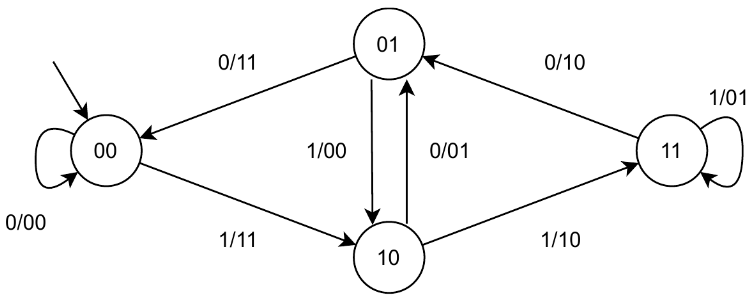
\includegraphics[scale=0.7]{convoluzionatore_1_2_fsm.png}
    \caption{FSM convoluzionatore $1/2$}
    \label{fig:fsm_conv}
\end{figure}

Il modulo deve quindi restituire in output (scrivendo in memoria) le uscite della macchina a stati finiti,
bit per bit. % dire meglio

\subsection{Esempio}

La FSM prende in input la parola \verb+11001011+, che deve essere serializzata come
1 al tempo 0, 1 al tempo 1, 0 al tempo 2 e così via.
La macchina quindi, partendo dallo stato di reset 00 andrà nello stato 10 alla lettura
del primo 1 producendo in output 11, passerà poi nello stato 3 producendo 10, nello stato 01
producendo 10 e nello stato 00 producendo 11.
Il primo byte di output sarà quindi 11100111, che dovrà essere scritto in memoria.
Si nota quindi facilmente che la lunghezza della sequenza di output è esattamente doppia di quella 
dell'input.

\pagebreak

\subsection{Specifiche del modulo da realizzare}

Il modulo da descrivere è sincrono sincronizzato su un clock 'globale', non include la memoria su cui viene effettuato input/output e
deve implementare la seguente interfaccia verso l'esterno:

\begin{minted}[]{vhdl}
    
    entity project_reti_logiche is
        port (
            i_clk : in std_logic;
            i_rst : in std_logic;
            i_start : in std_logic;
            i_data : in std_logic_vector(7 downto 0);
            o_address : out std_logic_vector(15 downto 0);
            o_done : out std_logic;
            o_en : out std_logic;
            o_we : out std_logic;
            o_data : out std_logic_vector (7 downto 0)
        );
    end project_reti_logiche;

\end{minted}

In particolare:

\begin{itemize}
    \item \texttt{i\_clk} è il segnale di clock, generato dall'esterno
    \item \texttt{i\_rst} è il segnale di reset
    \item \texttt{i\_start} è il segnale di inizio sequenza
    \item \texttt{i\_data} è il byte in arrivo dalla memoria
    \item \texttt{o\_address} è l'indizzo di memoria da cui si vuole leggere/scrivere
    \item \texttt{o\_done} è il segnale di fine computazione
    \item \texttt{o\_en} è il segnale di enable per la memoria
    \item \texttt{o\_we} è il segnale di scrittura per la memoria
    \item \texttt{o\_data} è il byte da scrivere in memoria
\end{itemize}

\end{document}